% ============================================================================
% CHAPTER 5 — GA-SLM: GENETIC ALGORITHM-ENHANCED SLM
% ============================================================================
\chapter{GA-SLM: Genetic Algorithm-Enhanced SLM}
\label{ch:ga_slm}

\begin{motivation}
    PRNet and NN-SCF replace the SLM search entirely with a neural network.
    But what if we want to \emph{keep} the SLM framework and simply make its
    phase-sequence search smarter?
    Ali et al.\ (2016) proposed using a \textbf{Genetic Algorithm (GA)} to
    optimize the SLM phase sequences, achieving near-optimal PAPR reduction
    without exhaustively testing all $U$ candidates.
    This is the only approach in our survey that does not use neural
    networks---it applies evolutionary optimization directly to
    the SLM problem~\cite{ali2016new}.
\end{motivation}


% ----------------------------------------------------------------------------
\section{Conceptual Overview}
\label{sec:gaslm_concept}
% ----------------------------------------------------------------------------

Recall from Chapter~\ref{ch:refresher} that classical SLM generates $U$
candidate signals by applying $U$ fixed phase sequences to the data, then
selects the candidate with the lowest PAPR.  The problem is that $U$
phase sequences explore only a tiny fraction of the vast phase-sequence
space.  To achieve better PAPR reduction, we need more candidates---but
each candidate requires an additional IFFT~\cite{ali2016new}.

The GA-SLM approach resolves this by using a Genetic Algorithm to
\textbf{intelligently search} the phase-sequence space without exhaustive
enumeration.  Instead of pre-defining $U$ fixed sequences, the GA
\emph{evolves} a population of phase sequences over multiple generations,
converging toward the sequence that minimizes PAPR for the \emph{current}
OFDM symbol~\cite{ali2016new}.

\begin{keyinsight}
    The fundamental difference between GA-SLM and the neural network
    approaches is the timing of optimization.
    Neural networks train \emph{offline} (once, before deployment) and
    run fast inference \emph{online}.
    The GA optimizes \emph{online}---it runs a full evolutionary search
    for \emph{each} OFDM symbol at transmission time.
    This gives the GA access to symbol-specific optimization but at the
    cost of higher per-symbol latency~\cite{ali2016new}.
\end{keyinsight}


% ----------------------------------------------------------------------------
\section{System Model}
\label{sec:gaslm_system}
% ----------------------------------------------------------------------------

\subsection{OFDM Signal with SLM Phase Rotation}

The OFDM signal after IFFT with $N$ subcarriers is~\cite{ali2016new}:
\begin{equation}
    x(n) = \frac{1}{\sqrt{N}} \sum_{k=0}^{N-1} X_k \, e^{\,j2\pi kn/N},
    \qquad n = 0, 1, \dots, N-1.
    \label{eq:gaslm_ofdm}
\end{equation}

In SLM, each candidate signal is generated by multiplying the data by a
phase sequence $\bm{\psi}_u$ before the IFFT.
The PAPR of the $u$-th candidate is~\cite{ali2016new}:
\begin{equation}
    \mathrm{PAPR}_u
    = \frac{\displaystyle\max_{n}\left|\frac{1}{\sqrt{N}}
    \sum_{k=0}^{N-1} X_k \psi_{u,k}\, e^{\,j2\pi kn/N}\right|^2}
    {E\!\left[\left|\frac{1}{\sqrt{N}}
    \sum_{k=0}^{N-1} X_k \psi_{u,k}\, e^{\,j2\pi kn/N}\right|^2\right]}.
    \label{eq:gaslm_papr}
\end{equation}

\begin{figure}[H]
    \centering
    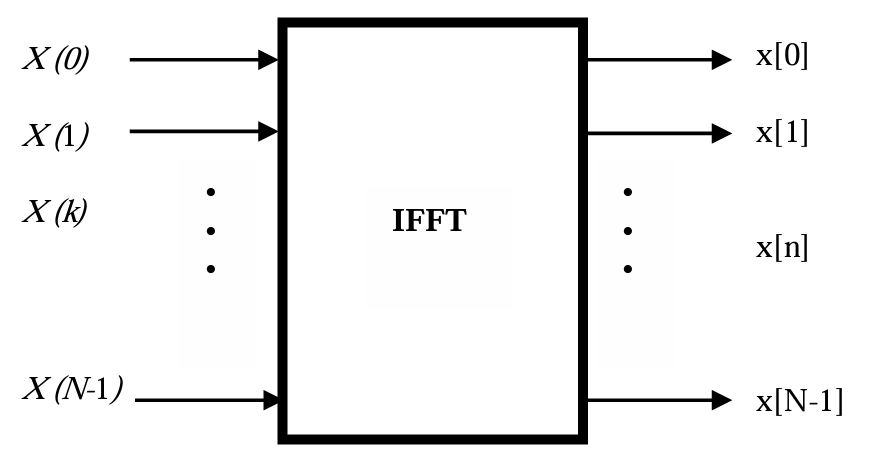
\includegraphics[width=0.50\linewidth]{Figures/22_ifft_ofdm_symbol.png}
    \caption{IFFT-based OFDM signal generation.
             Each subcarrier carries a modulated symbol $X_k$; the IFFT
             produces the time-domain signal $x(n)$.
             Reproduced from~\cite{ali2016new}.}
    \label{fig:ifft_ofdm}
\end{figure}

\begin{figure}[H]
    \centering
    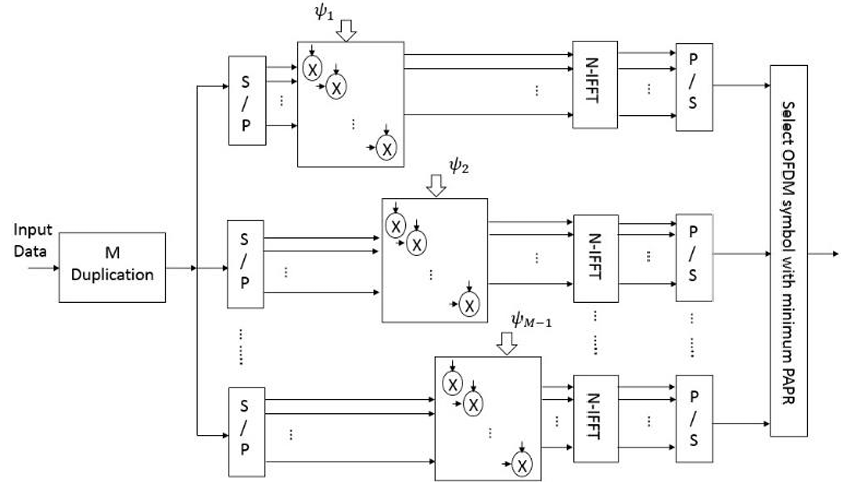
\includegraphics[width=0.85\linewidth]{Figures/23_slm_functional_diagram.png}
    \caption{Functional diagram of conventional SLM.
             Multiple phase sequences are applied before the IFFT, and the
             candidate with the lowest PAPR is selected for transmission.
             The selected phase index is sent as side information.
             Reproduced from~\cite{ali2016new}.}
    \label{fig:slm_functional}
\end{figure}


% ----------------------------------------------------------------------------
\section{The Genetic Algorithm for SLM}
\label{sec:gaslm_algorithm}
% ----------------------------------------------------------------------------

\begin{figure}[H]
    \centering
    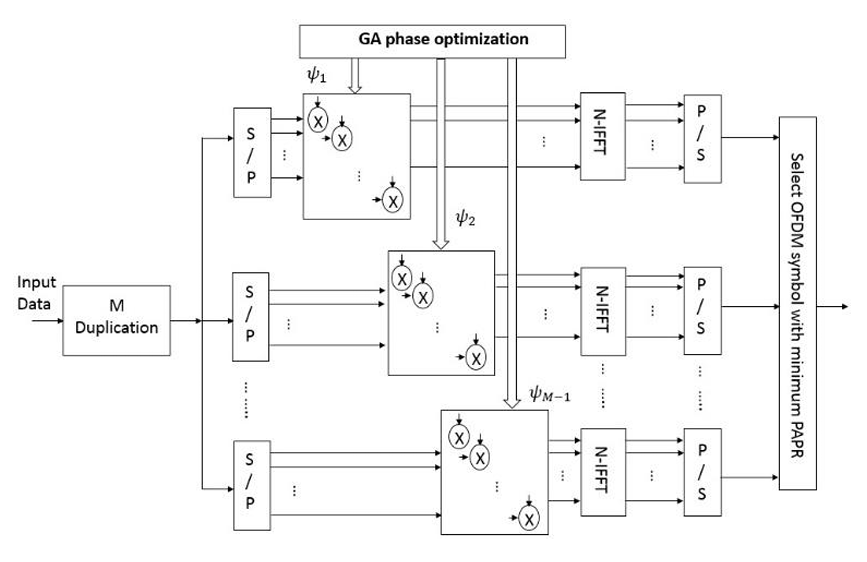
\includegraphics[width=0.85\linewidth]{Figures/24_ga_slm_block_diagram.png}
    \caption{Block diagram of the GA-based SLM scheme.
             The GA replaces the fixed phase-sequence set with an evolving
             population of candidates.  At each generation, the fittest
             (lowest-PAPR) individuals survive and produce offspring via
             crossover and mutation.
             Reproduced from~\cite{ali2016new}.}
    \label{fig:gaslm_block}
\end{figure}

\subsection{Encoding: Chromosome Representation}

Each candidate phase sequence is represented as a
\textbf{chromosome}~\cite{ali2016new}:
\begin{equation}
    \bm{\psi} = [\psi_0,\; \psi_1,\; \dots,\; \psi_{N-1}],
    \qquad \psi_k \in \{e^{j2\pi m/M} : m = 0, 1, \dots, M-1\},
    \label{eq:gaslm_chromosome}
\end{equation}
where $M$ is the size of the \textbf{phase alphabet}.
For $M = 2$, the phases are $\{+1, -1\}$ (binary encoding).
For $M = 4$, the phases are $\{+1, -1, +j, -j\}$~\cite{ali2016new}.

Each gene $\psi_k$ corresponds to the phase factor applied to the $k$-th
subcarrier.  With $N$ subcarriers and $M$ possible phases per subcarrier,
the total search space has $M^N$ elements---an astronomically large number
for even moderate $N$ (e.g., $2^{128} \approx 3.4 \times 10^{38}$ for
binary phases with $N=128$).  Exhaustive search is clearly
impossible~\cite{ali2016new}.

\subsection{Fitness Function}

The fitness function directly evaluates the PAPR achieved by each
chromosome~\cite{ali2016new}:
\begin{equation}
    \mathcal{F}(\bm{\psi})
    = -\mathrm{PAPR}\!\bigl(\mathrm{IFFT}\{\bm{X} \odot \bm{\psi}\}\bigr).
    \label{eq:gaslm_fitness_fn}
\end{equation}
The negative sign converts minimization of PAPR into maximization of fitness
(the conventional GA objective).

\subsection{Selection}

The selection operator chooses parent chromosomes for reproduction.
Ali et al.\ use \textbf{tournament selection}~\cite{ali2016new}:
randomly select a small subset (tournament) from the population,
and the individual with the highest fitness ``wins'' and becomes a parent.
This process is repeated to select pairs of parents for crossover.

\subsection{Crossover}

Two parent chromosomes exchange genetic material to produce offspring.
For SLM phase sequences, \textbf{single-point crossover} is
used~\cite{ali2016new}:
\begin{enumerate}
    \item Choose a random crossover point $c \in \{1, \dots, N-1\}$.
    \item The first offspring inherits genes $[\psi_0, \dots, \psi_{c-1}]$
          from parent~1 and $[\psi_c, \dots, \psi_{N-1}]$ from parent~2.
    \item The second offspring inherits the complementary combination.
\end{enumerate}

\begin{workingexample}[Crossover with $N=8$]
    Parent 1: $[+1, -1, +1, +1, \;|\; -1, +1, -1, +1]$

    Parent 2: $[-1, +1, -1, +1, \;|\; +1, -1, +1, -1]$

    Crossover point $c = 4$:

    Offspring 1: $[+1, -1, +1, +1, \;|\; +1, -1, +1, -1]$

    Offspring 2: $[-1, +1, -1, +1, \;|\; -1, +1, -1, +1]$

    Each offspring combines traits from both parents, potentially
    producing a phase sequence with lower PAPR than either parent.
\end{workingexample}

\subsection{Mutation}

To maintain genetic diversity and prevent premature convergence,
mutation randomly alters some genes in the offspring.  With probability
$p_m$ (the \textbf{mutation rate}), each gene $\psi_k$ is replaced by a
randomly chosen phase from the alphabet~\cite{ali2016new}:
\begin{equation}
    \psi_k^{\prime} =
    \begin{cases}
        \text{random phase from } \{e^{j2\pi m/M}\}, & \text{with probability } p_m, \\
        \psi_k, & \text{with probability } 1 - p_m.
    \end{cases}
    \label{eq:gaslm_mutation}
\end{equation}

\subsection{Complete GA-SLM Algorithm}

The full procedure for each OFDM symbol is~\cite{ali2016new}:

\begin{algorithm}[H]
\SetAlgoLined
\KwIn{OFDM data $\bm{X}$, population size $P$, generations $G$,
      crossover rate $p_c$, mutation rate $p_m$, phase alphabet size $M$}
\KwOut{Phase sequence $\bm{\psi}^*$ yielding minimum PAPR}

Initialize $P$ random phase sequences $\{\bm{\psi}_1, \dots, \bm{\psi}_P\}$\;
\For{$g = 1$ \KwTo $G$}{
    Compute fitness $\mathcal{F}(\bm{\psi}_i)$ for all $i = 1, \dots, P$
    (requires $P$ IFFT operations)\;
    Record the best individual (elitism)\;
    \For{$i = 1$ \KwTo $P/2$}{
        Select two parents via tournament selection\;
        With probability $p_c$, perform single-point crossover
        to generate two offspring\;
        Apply mutation with rate $p_m$ to each offspring\;
        Add offspring to the new population\;
    }
    Replace the old population with the new one
    (keeping the elite individual)\;
}
\Return{best individual $\bm{\psi}^* = \arg\max_i \mathcal{F}(\bm{\psi}_i)$}\;
\caption{GA-SLM Phase Sequence Optimization~\cite{ali2016new}}
\label{alg:gaslm}
\end{algorithm}


% ----------------------------------------------------------------------------
\section{Simulation and System Parameters}
\label{sec:gaslm_params}
% ----------------------------------------------------------------------------

\begin{table}[H]
    \centering
    \caption{Simulation parameters for GA-SLM~\cite{ali2016new}.}
    \label{tab:gaslm_params}
    \begin{tabular}{@{} l l @{}}
        \toprule
        \textbf{Parameter} & \textbf{Value} \\
        \midrule
        Number of subcarriers ($N$) & 128 \\
        Modulation scheme & QPSK \\
        Phase alphabet size ($M$) & 2 (binary: $\{+1, -1\}$) \\
        Population size ($P$) & 20--150 \\
        Number of generations ($G$) & 10--500 \\
        Crossover type & Single-point \\
        Crossover rate ($p_c$) & 0.8 \\
        Mutation rate ($p_m$) & 0.01--0.05 \\
        Selection method & Tournament selection \\
        Elitism & Yes (best individual preserved) \\
        Number of OFDM symbols & $10^4$ \\
        Oversampling factor & 4 \\
        \bottomrule
    \end{tabular}
\end{table}


% ----------------------------------------------------------------------------
\section{Results and Analysis}
\label{sec:gaslm_results}
% ----------------------------------------------------------------------------

\subsection{CCDF Performance}

\begin{figure}[H]
    \centering
    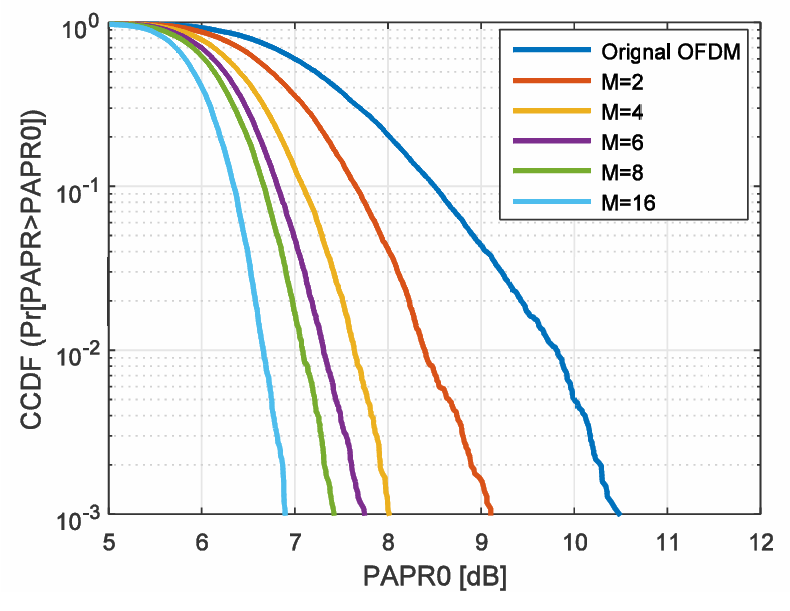
\includegraphics[width=0.65\linewidth]{Figures/25_slm_ccdf.png}
    \caption{CCDF of the OFDM for conventional SLM technique with different numbers
             of phase sequences $M$ and $N=128$ subcarriers. Shows the diminishing returns
             of increasing $M$ in standard SLM.
             Reproduced from~\cite{ali2016new}.}
    \label{fig:slm_ccdf}
\end{figure}

\begin{figure}[H]
    \centering
    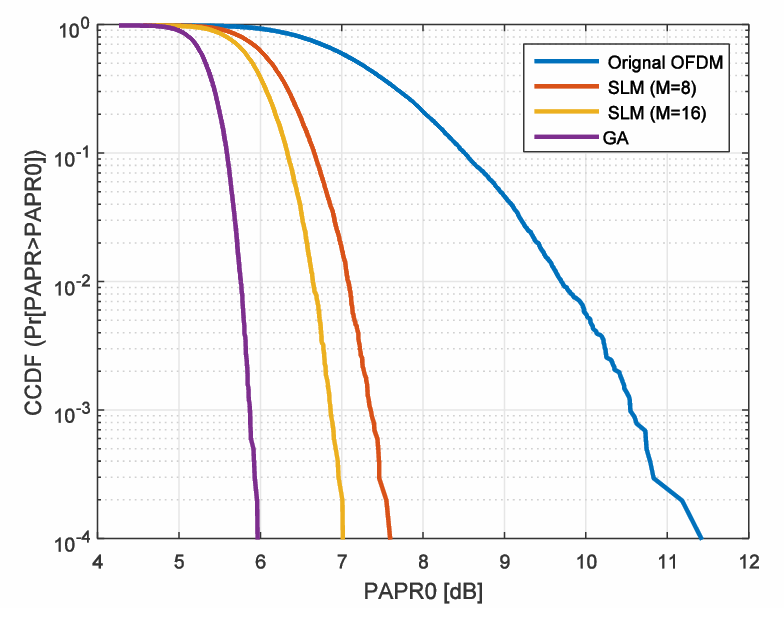
\includegraphics[width=0.65\linewidth]{Figures/26_ga_slm_ccdf_comparison.png}
    \caption{CCDF of the original OFDM, GA-based SLM, and conventional SLM
             techniques for $M=8, 16$. GA-based SLM achieves superior PAPR
             reduction compared to conventional SLM with the same number of IFFT evaluations.
             Reproduced from~\cite{ali2016new}.}
    \label{fig:gaslm_ccdf}
\end{figure}

\begin{keyinsight}
    The GA-SLM can achieve PAPR reduction equivalent to conventional SLM
    with $U=16$ candidates while evaluating far fewer candidates through
    intelligent search.  The GA effectively ``explores'' the phase-sequence
    space much more efficiently than random sampling~\cite{ali2016new}.
\end{keyinsight}

\subsection{Effect of Population Size}

\begin{figure}[H]
    \centering
    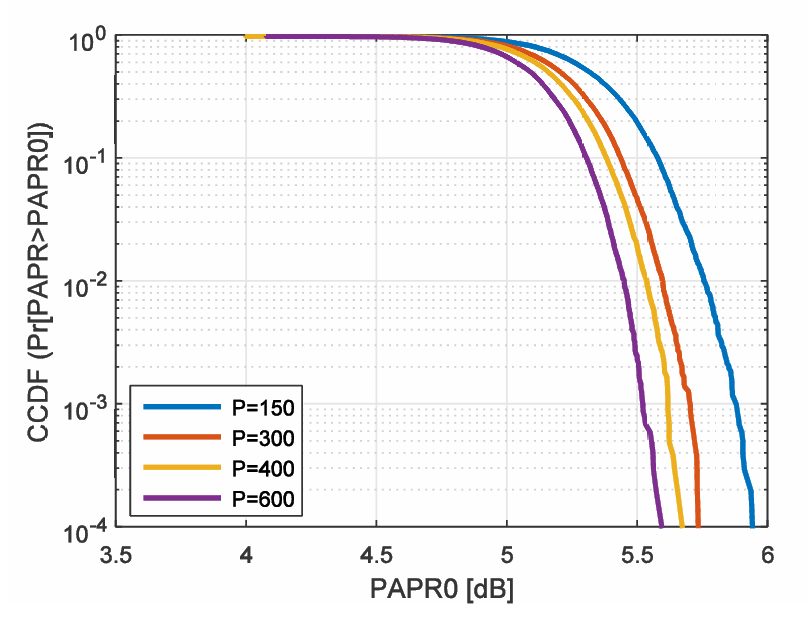
\includegraphics[width=0.65\linewidth]{Figures/27_ga_slm_population.png}
    \caption{CCDF of PAPR for GA-SLM with different population sizes $P$.
             Larger populations provide better exploration of the search
             space but require more IFFT computations per generation.
             Reproduced from~\cite{ali2016new}.}
    \label{fig:gaslm_population}
\end{figure}

\subsection{Convergence vs.\ Number of Iterations}

\begin{figure}[H]
    \centering
    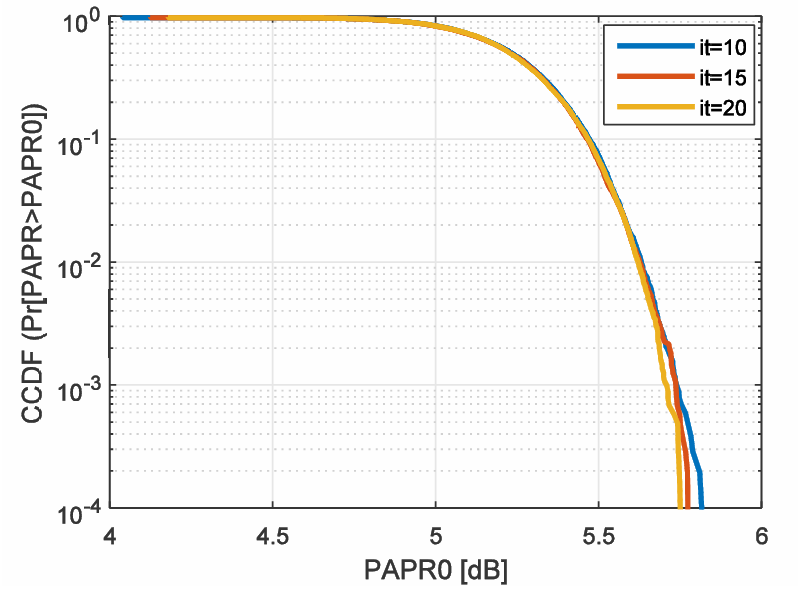
\includegraphics[width=0.60\linewidth]{Figures/28_ga_slm_iterations.png}
    \caption{PAPR reduction as a function of the number of GA generations.
             Most of the improvement occurs within the first 50--100
             generations, with diminishing returns afterward.
             Reproduced from~\cite{ali2016new}.}
    \label{fig:gaslm_iterations}
\end{figure}


% ----------------------------------------------------------------------------
\section{Complexity Analysis}
\label{sec:gaslm_complexity}
% ----------------------------------------------------------------------------

The computational complexity of GA-SLM per OFDM symbol is
proportional to the total number of fitness evaluations~\cite{ali2016new}:
\begin{equation}
    \mathcal{C}_{\mathrm{GA\text{-}SLM}}
    = P \times G \times \mathcal{O}(N \log_2 N).
    \label{eq:gaslm_complexity}
\end{equation}

Each fitness evaluation requires one $N$-point IFFT, and there are $P$
individuals evaluated over $G$ generations.

\begin{workingexample}[Complexity Comparison]
    For $N=128$, $P=20$, $G=100$:
    \begin{itemize}
        \item GA-SLM: $20 \times 100 = 2000$ IFFT operations per symbol.
        \item Conventional SLM with $U=16$: only 16 IFFT operations.
    \end{itemize}
    The GA-SLM requires $125\times$ more computation than $U=16$ SLM!
    However, the PAPR reduction achieved is significantly better
    because the GA explores many more phase sequences
    intelligently~\cite{ali2016new}.
\end{workingexample}

\begin{misconception}
    \textbf{``GA-SLM reduces computational complexity compared to SLM.''} \\
    This is incorrect.  GA-SLM typically requires \emph{more} total IFFT
    operations than conventional SLM.  Its advantage is achieving
    \emph{better PAPR reduction} for a given target, or achieving the
    \emph{same PAPR reduction} with fewer total evaluations than
    would be needed by exhaustive search over $M^N$ possible
    sequences~\cite{ali2016new}.
\end{misconception}


% ----------------------------------------------------------------------------
\section{Limitations and Open Problems}
\label{sec:gaslm_limitations}
% ----------------------------------------------------------------------------

\begin{enumerate}
    \item \textbf{High per-symbol latency:}
          Running $P \times G$ IFFT operations for every OFDM symbol
          introduces significant processing delay, potentially
          incompatible with real-time requirements~\cite{ali2016new}.

    \item \textbf{No offline training:}
          Unlike neural network approaches, the GA cannot amortize its
          computational cost through offline training.  Every symbol
          requires a fresh optimization run.

    \item \textbf{Side information still required:}
          The receiver still needs to know which phase sequence was
          selected, requiring $\lceil\log_2 P\rceil$ SI bits (or a
          blind detection mechanism)~\cite{ali2016new}.

    \item \textbf{No BER guarantee:}
          The GA does not explicitly optimize for BER; it only
          minimizes PAPR.  However, since SLM is distortion-free
          (phase rotations are reversible), the BER should be
          unaffected if SI is received correctly.

    \item \textbf{Stochastic behavior:}
          The GA is inherently random---different runs on the same
          OFDM symbol may produce different results.
\end{enumerate}


% ----------------------------------------------------------------------------
\section{Connection to Other Approaches}
\label{sec:gaslm_connections}
% ----------------------------------------------------------------------------

GA-SLM occupies a unique position in our landscape of ML-enhanced SLM
techniques:
\begin{itemize}
    \item It is the \textbf{only non-neural-network} approach, demonstrating
          that ML-enhanced PAPR reduction does not necessarily require
          deep learning.
    \item It \textbf{preserves the SLM framework} entirely, merely
          replacing the phase-sequence selection strategy.
    \item It \textbf{optimizes per-symbol} rather than pre-training once,
          making it the most adaptable but also the most computationally
          expensive approach at runtime.
\end{itemize}

The next chapter examines Hao et al.'s ESLM-AE, which takes the opposite
approach: it uses an autoencoder to \emph{learn} the optimal phase factors
once during training, enabling fast inference with no per-symbol
search~\cite{hao2019extended}.
